\documentclass{article}
\usepackage[utf8]{inputenc}
% formatting imports
\usepackage{graphicx}
\usepackage[margin=1cm]{caption}
\usepackage[a4paper, total={6in, 8in}]{geometry}
\usepackage[section]{placeins}
\usepackage{array}

\usepackage{setspace}

% math imports
\usepackage{siunitx}
\usepackage{amsmath}
\usepackage{amsthm}
\usepackage{amssymb}
\usepackage{mathtools}
\usepackage{bbold}

\usepackage{listings}
\lstset{basicstyle=\footnotesize\ttfamily,breaklines=true}
\lstset{framextopmargin=50pt,frame=bottomline}


\usepackage[textsize=tiny]{todonotes}
\usepackage{longtable}

\usepackage[sorting=none]{biblatex}
\addbibresource{refs.bib}

\newcommand{\todoref}[2][]{\todo[color=cyan!40, #1]{\textbf{add ref:}\\#2}}
\newcommand{\todofig}[2][]{\todo[color=red!40, #1]{\textbf{add fig:}\\#2}}
\newcommand{\todoidea}[2][]{\todo[color=green!40, #1]{\textbf{idea:}\\#2}}
\newcommand{\todoexplain}[2][]{\todo[color=purple!40, #1]{\textbf{add details:}\\#2}}

\usepackage{subfigure}
% green!40]

\usepackage[fontsize=12pt]{fontsize}

\newcommand{\del}[2]{\frac{\partial #1}{\partial #2}}
\newcommand{\delsquare}[2]{\frac{\partial^2 #1}{\partial #2 ^2}}

\newcommand{\full}[2]{\frac{d #1}{d #2}}
\newcommand{\fullsquare}[2]{\frac{d^2 #1}{d #2 ^2}}

\newcommand{\ccf}[1]{`\textsf{#1}'}
\newcommand{\cf}[1]{\textsf{#1}}

\title{IGNORE THIS PAGE IN CURRENT VERSION}

\DeclareUnicodeCharacter{2212}{-}
\begin{document}

\listoftodos

\doublespacing

% \maketitle

% \begin{center}
%     Massachusetts Institute of Technology \\
%     Department of Electrical Engineering and Computer Science
% \end{center}

% \begin{center}
%     Proposal for Thesis Research in Partial Fulfillment\\ of the Requirements for the Degree of\\
% Masters of Engineering
% \end{center}

% \vfill

% \begin{tabular}{rl}
% \textbf{Title:} & \textbf{Defect Identification in Superconducting 2-Terminal Devices} \\
% \\
% \textbf{Submitted by:} & T. Dandachi \\
%               & 69 Chestnut St. \\
%               & Cambridge, MA 02139
% \end{tabular}

% \vspace{15mm}
% \begin{tabular}{@{}p{1.5in}p{4in}@{}}
% \textbf{Signature of author:} & \hrulefill \\
% \end{tabular}

% \vfill

% \textbf{Expected Date of Completion:} May 2022

% \vfill

% \textbf{Laboratory:} Quantum Nanostructures and Nanofabrication under the Research Laboratory for Electronics

% \vfill

% \textbf{Abstract:}

% Simulating the operation of a superconducting device

% \vfill

% \textbf{Supervision Agreement:}

% The program outlined in this proposal is adequate for a Master's thesis. The supplies and facilities required are available, and I am willing to supervise the research and evaluate the thesis report.

% \vspace{15 mm}
% \begin{tabular}{@{}p{1.5in}p{4in}@{}}
%   & \hrulefill \\
% & K. K. Berggren, Prof. of Elec. Eng.
% \end{tabular}

% \newpage

\tableofcontents

\newpage

% figures are here: https://www.icloud.com/keynote/094kHrSTQlvohxqCHGUmZJXcg#thesis

\section{Introduction}

The non-linearity exhibited by superconducting nanowires is of key importance to many of its applications,
from superconducting nanowire single-photon detectors (SNSPDs) to neuromorphic computing. This non-linearity
however is also the reason simulating nanowires is an increasingly hard problem, especially when we start
to care about the microwave properties of these devices. A common way of simulating these nanowire electronics
builds on top of existing circuit simulation environments that were optimized for classical electronics -- where
the microwave and superconducting properties of the models did not matter. 

Simulating the predominant effects in our superconducting electronics is an important step in designing
superconducting devices.

While the requirement for better nanowire simulations and the complexity of our models are steadily increasing,
the tools used to simulate

Sending pulses is cool

\todo[inline]{not done}

\subsection{Non-linearity in superconducting nanowires}

Superconducting nanowires are highly non-linear and present three main forms of non-linearity:
kinetic inductance, state transitions between the normal and superconducting state and
coupling to other non-linear dynamics.

Kinetic inductance is a continuous form of non-linearity introduced by the inertia of cooper
pairs in a nanowire. In thin films, kinetic inductance is highly dependent on the film thickness,
temperature, and magnetic field \cite{dizhu-thesis}. In nanowires, the effect of a bias current
on the kinetic inductance is a well-studied phenomenon. Of particular interest to more complicated
electronics and SNSPDs is the ability to simulate the effects of pulses and non-DC current behavior
on the kinetic inductance. This is an important effect since the non-linearity of some nanowire 
geometry can change the shapes of pulses traveling in the nanowire. This causes even simple designs 
such as a superconducting transmission line operating only in the superconducting regime to 
behave in a difficult to anticipate non-linear fashion. 

The second form of non-linearity pertains to the superconducting state. By assuming the device is
experiencing a constant magnetic field and temperature, we can find a threshold critical current,
$i_c$, where if the current exceeds that value locally along a nanowire, it switches out of the 
superconducting state and into the resistive state. This switching behavior is a non-linearity
over a boolean state that is dependent on the current flowing through each portion of the nanowire.
Non-linearities over a boolean state are particularly hard to simulate as they involve sudden large
magnitude changes. Typical non-linear solvers are optimized for continuous non-linear systems where
the solver enters a loop making the timestep smaller until the magnitude of change is small.
In boolean states, there is no sense of continuity, and in the limit of smaller timesteps, the 
change in response magnitude will be just as large. 

\subsection{Nanowire Elements}

From an electronics standpoint, a nanowire's lumped model is a non-linear inductor when superconducting. When resistive, an additional resistor is in series with that inductor.
These two building blocks (a continuously non-linear inductor and a discrete non-linear
resistance) are the basis for modeling the behavior of superconducting nanowires in
the electronics picture and cover the two main types of non-linearities exhibited.

A more complicated - but necessary - picture includes coupling to a thermal equation.
A nanowires critical temperature $i_c$ and critical temperature $T_c$ are in reality
functions of the current state of the superconductor, they are related by the critical
surface, $T_c(i=0) \neq T_c(i=0.75i_c)$. The superconducting-to-normal state transition
begins a coupled chain reaction between a thermal system and an electrical system, making
modeling nanowires harder. When a portion of the nanowire switches into the resistive 
state, a normal region starts to form in the wire that dissipates thermal energy. This
energy heats up the surrounding portions of the nanowire, decreasing their critical 
current. At the same time, the normal region has a higher impedance than the nanowire
diverting current around it, allowing portions of the nanowire to see a higher density of
the current, making it more likely to switch in the plane of the hotspot. The hotspot also
dissipates heat to the stack and fridge. These are well-studied phenomena for nanowires
and tend to be modeled through experimentally fitted parameters for the electrical-thermal
coupling. \todoexplain[]{maybe talk about simulating noise transition??}\todoref[]{ref karl nanowire. ref others??}

Another picture that tends to be neglected is the distributed picture of the nanowire.
In reality, the nanowire has a spatial dimension to it and is a microwave device. This
picture tends to enforce simulation constraints as the discretization and network size
increase. This picture accounts for time delays introduced for a signal entering and
leaving a nanowire, resonances that might occur in the nanowire, as well as distributed
thermal and electrical effects that don't make sense in the lumped picture. For meanders
longer than the wavelength of frequencies carried, modeling them as distributed devices
is essential. Not doing so can result in the device not switching when it has to. Another
big effect that can't be captured with non-distributed pictures is pulse reshaping, more
on that in Section \ref{tapers_intro}.


\todoidea[inline]{tlines}
\todofig[]{tline fig}

\todoidea[inline]{CPW geometry}

\todoref[inline]{ref https://arxiv.org/pdf/1805.05601.pdf}


\missingfigure[]{nanowire model simple circuit}

\subsubsection{SNSPDs}

One geometry a nanowire can be designed for are superconducting nanowire 
single-photon detectors (SNSPDs). By having a nanowire meander biased near
its critical current, a small energy perturbation (such as photon incidence)
cause a transition into the normal state. As a result a single photon injecting
a small amount of energy into the nanowire has an amplified output from the bias 
current flwoing across no resistor to a large resistor (usually on the order of 
$1k\Omega$).\todoref{refernece for snspds}

For simple SNSPD designs, it is enough to model the device using a lumped element model
nanowire in parallel with a shunt resistor.
Assuming an SNSPD with $50\Omega$ impedance shunted with a $50\Omega$ resistor, in this 
topology, the current is split and equally diverted into the shunt and nanowire.
If biased at the right threshold, a photon count would correspond to a tiny spike in 
the current flowing through the nanowire leading to a switching event. The nanowire 
produces a voltage pulse as a $\sim 7k\Omega$ resistor forms (this number is dependent on
multiple design parameters). Due to the impedance mismatch,
the current prefers the shunt resistor branch, which allows the hotspot to cool off
and resets the SNSPD.

\todofig[]{typical snspd readout setup figure}

\subsubsection{SNSPIs}

Superconducting nanowire single-photon imagers (SNSPIs) are used in a similar fashion
to SNSPDs but take advantage of the distributed picture for larger lengths of nanowire.
SNSPIs tend to be be designed to have a slower propagation velocity and longer meanders.
These effects cause a switching effect in the wire to take time to propagate to the two 
ends of the nanowire. By differentially reading out the meander, we can spatially resolve
the photon incidence location as a function of the delay between the 2 ports of the SNSPI.

In this image, the SNSPI can be thought of as a non-linear transmission line that
has both the non-linearities described above. By discretizing the transmission line
into multiple lumped elements, the local non-linear contributions can be modeled by a
non-linear inductor and resistor, while keeping the capacitor linear. In this image,
this can be thought of as a long chain of discrete lumped nanowire elements in parallel
with linear capacitor elements. This topology captures the distributed picture of
pulses propagating in nanowire meanders and allows us to simulate SNSPIs.

\subsubsection{Impedance Matching Tapers} \label{tapers_intro}

Usually the nanowire's impedance is not similar enough to that of the input and output circuitry. This mismatch causes the signal to reflect back into the wire instead 
of propagating into the next stage, causing interference and distortions. Impedance 
matching is done by designing tapers: extensions of the same line that increase in 
width slowly as shown in figure \ref{fig:wirematlab}. This slow increase ensures 
that there is minimal step change in impedance allowing for less reflections on the 
impedance boundaries. A Klopfenstein taper is the optimal taper geomtery for its length
in decreasing the total amount 
of reflections \cite{klopfenstein_transmission_1956}\todoref{cite klopf}. 
The slow change in width still causes internal reflections along the length of the 
wire, however, their overall magnitude is smaller than one step change as illustrated in 
figure \ref{fig:whatsataper}.
\todoidea[inline]{mayhaps exponential taper, etc.}

Impedance matching tapers are often used on nanowire devices when we care about preseving
the signal shape and magnitude allowing us to use the SNSPDs readout pulses in more
interesting ways and preserve logic pulses. Impedance matching tapers allow us to
perform photon number resolution - infer the number of incident photons on a nanowire
from the readout pulse as shown in more details in section \ref{tapers_section}.
In devices like SNSPIs, the reflections caused by impedance mismatch at the edges can
prohibit us from timing the pulses correctly and as a result spatially resolving the
photon. This can also be remedied by the introduction of a taper.
\todoref[]{marco's snspd paper}\todoref[]{DiZhu MW paper}\todoref[]{taper on SNSPI?}

\begin{figure}[h]
    \centering
  \subfigure[]{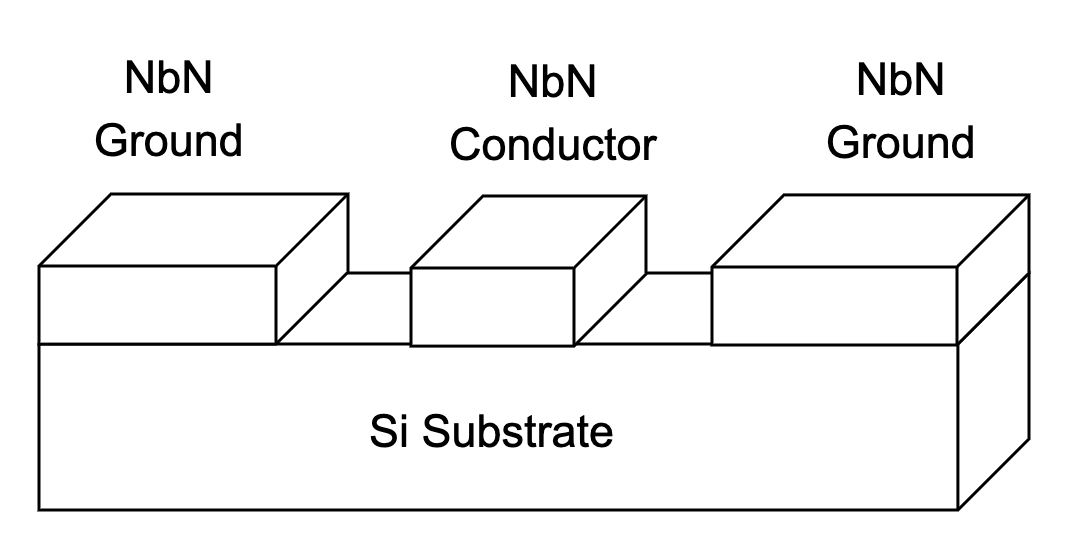
\includegraphics[width=0.35\textwidth]{figs/layers.png}\label{fig:cpwlayers}}
  \subfigure[]{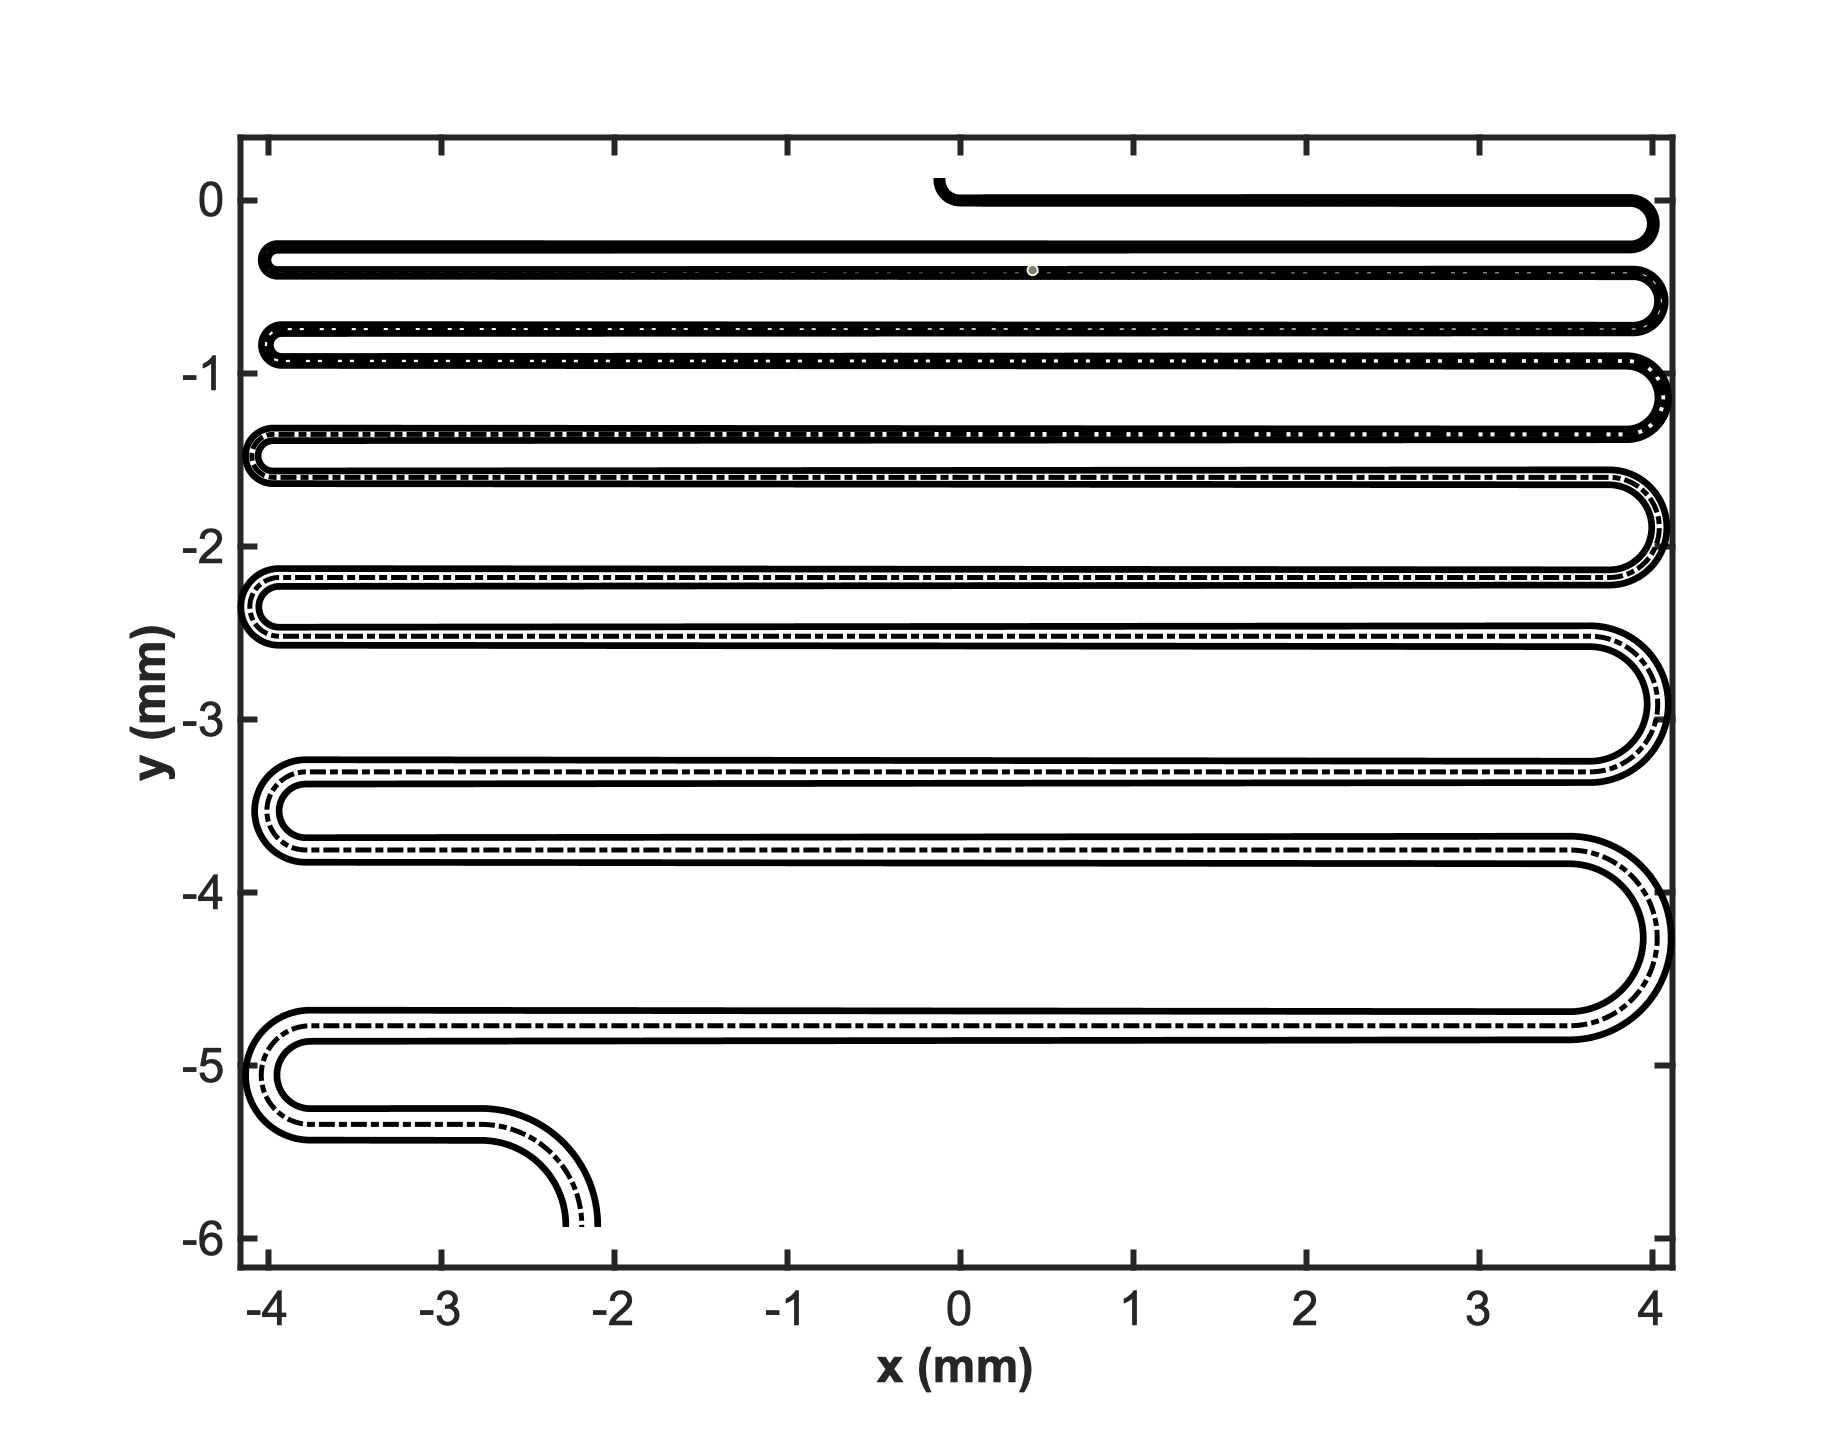
\includegraphics[width=0.5\textwidth]{figs/wire_matlab.png}\label{fig:wirematlab}}
    \caption{(a) Vertical slice a Co-Planar Waveguide (CPW) geometry for a Niobium Nitride (NbN) nanowire. (b) Top view of a Klopfenstein taper with a folded meander.\todofig[inline]{Forgot a layer lol}}
    \label{fig:thewiredesign}
\end{figure}

\begin{figure*}[h]
  \centering
  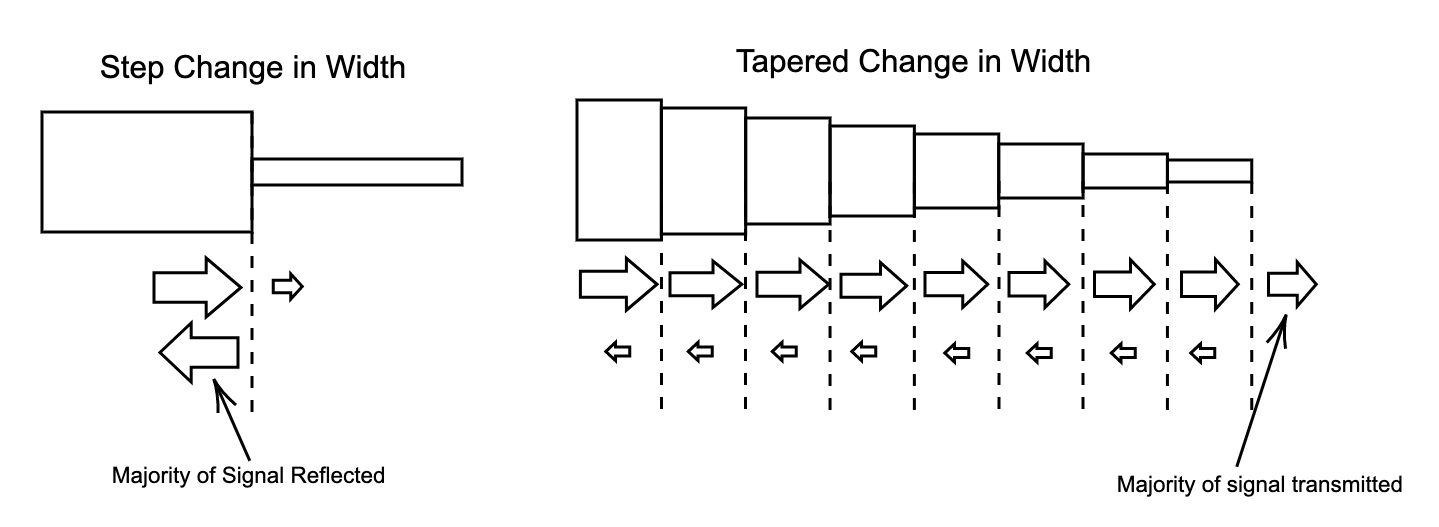
\includegraphics[width=5in]{figs/whatsataper.png}
  
  \caption{A tapered change in width causes smaller reflections at each boundary which add up to a lower total amount of reflection than a singular step change in width. Change in width is roughly proportional to change in impedance. The inclusion of multiple step changes in
  width increases the number of individual reflections occurring step
  and the number of interferences a simulator would need to keep track of grows 
  exponentially increasing the complexity of the simulation.}
 \label{fig:whatsataper}
\end{figure*}

One side effect of using a Klopfenstein taper is the change in propagation velocity caused by the change of electrical characteristics in the wire. Using $L(x)$ and $C(x)$ as the inductance and capacitance along the length of the wire, 
the continuous version of equation 1b\todo[]{place tline v prop eq in nanowire section...}
that $v_{p}(x)$ is dependant on $L\cdot C$. The Klopfenstein does not scale $L$ and $C$ inversely, which means that $v_{p}(x)$ is not constant along the wire. Coupling this with the fact that the thinner wire will have a higher current density, this becomes a huge source of distortion.

Long taper meander are folded into strips of straight wires connected by curved edges with 
large radii. This curvature is chosen in a manner that minimizes the amount of reflections
and current crowding: an unwanted effect caused by non-homogenous distributions 
of current density through a conductor that change the frequency response and impedance 
of the wire.\cite{hazra_superconducting_2016} Impedance matching and the folding of 
the wire both introduce distortions 
to the input signal and require the simulator to account for them.

\subsubsection{hTron}

Since the nanowire is also a thermal system that can generate heat and has its accessible state 
space affected by its current thermal state, modeling its thermal behavior is important for
accurate characterization. A CPW geometry nanowire, as shown in figure \ref{fig:cpwlayers}, consists 
of multiple layers. Having multiple layers of devices stacked on-top of each other can cause thermal
coupling between the devices.

While this coupling can be unwanted, devices that take advantage of that exist to create a new
set of superconducting circuits. One such device is the heater-tron (hTron)\todoref{htron!}. 
A simple device topology that uses the hTron is having two superconducting stacks separated
by an insulating layer. One of the stacks contains a resistor that generates heat while the
other stack contains a nanowire above the resistor. When current flows through the resistor
it generates heat that gets transmitted through the stack to the nanowire. Through this thermal
coupling, the nanowire can be thermally biased.

Simulating heat transport in stacks

\subsection{Problems Simulating Nanowires}

A full-model that simulates all the dynamics of superconducting nanowires is hard to achieve
due to the complexity, long simulation time, convergence issues and experimental fitting.
Previous parts of this section demonstrated multiple regimes nanowires can be used in,
from thermal coupling to a distributed microwave picture, each of which involves solving
stiff non-linear differential equations in the time domain. Getting a model to simualte
the electro-thermal coupling of a nanowire with respect to the stack, noise and photons
as well as the distributed effect accounting for non-linearities results in stiff non-linear
equations. As a result of this complexity, work is usually done on the individual parts
with experimental fits for each picture but no conception of the greater picture of how these
systems interact. This, in part, is also due to having multiple hard to define models for
each device topology that look different even though the fabricated device is identical.

Berggren et al. implemented a nanowire model in LTspice based on the phenomenological hotspot 
velocity model by Kermal et al. This model is a lumped element nanowire model that accounts 
for the hotspot dynamics with experimentally fitted parameters. It is implemented in LTspice
and contains both non-linearities exhibited by a nanowire using integrators and state saving,
discussed in more depth in section \ref{stability}.\todoref[]{karl spice} This model only 
accounts for the small signal solution and cannot be used in noise, AC or DC analysis.
The model also suffers from instability around the non-linearities. The instability and 
simulation modes are further discussed in section \ref{current_nw}.

Simulating tapers made out of the superconducting material cause the pulse to reshape,
an effect that isn't modeled in nanowire tapers.\todoref[]{idk?} Pulses traveling
in a taper experience reshaping due to the linear taper aspect, the change in impedance
reflects certain components from the pulse while leaving other frequencies untouched.
This reshaping can be completely captured by the scattering parameters and linear 
transmission lines. However, linear parameters do not account for non-linear reshaping
that is caused by kinetic inductance. Modeling tapers in LTspice tends to use a
sequence of transmission lines (namely the lossy transmission line model with $R=0$, 
discussed in \ref{tapers_section}) in series that have decreasing impedance. This model
is sufficient in simulating the linear part of the reshaping under the assumption
that the current flowing in the taper is much lower than the critical current, or
that in the DC picture, this effect reaches equilibrium and causes a final shift in the
perceived critical current of the device. In reality, this is not accurate, as pulses
being carried down a biased line also exhibit non-linear reshaping and this method
cannot be used to simulate pulse shapes accurately.

Non-linear simulation in superconductors has been studied a lot in the frequency domain
using techniques like Harmonic Balance. These methods can account for the continuous 
non-linearity presented by kinetic inductance, but not the state transition non-linearity.
JosephsonCircuits.jl for instance is designed
to simulate JTWPA topologies in the frequency domain using Harmonic Balance. WRspice
and Xyce both have Harmonic Balance backends that are very efficient. However,
for topologies that utilize the binary state non-linearity, time-domain simulation 
is needed to characterize the device behavior. Given the nature of WRspice and Xyce,
this implies that the entire circuit must be simulated in the time-domain. This is
addressed in section \ref{julia-sim-hb}.

The non-linearity of the electrical model gets even harder to simulate when coupled to
a thermal equation. As a result, the thermal coupling is usually linearized around the 
regime we care about. For example, for nanowires that have no need to thermally
interact with other elements, the hotspot growth is simulated via the phenomenological
hotspot velocity model \ref{matteo}\todoref[]{phen model}. 
For geometries that rely on thermal coupling such as the hTron, the critical current
of the device is presumed to be a function of the electron temperature \ref{matteo}.
\todoref[]{matteos thesis}
These models are sufficient but don't encompass a full thermal image of the device,
neglecting the thermal coupling that might occur between two nanowires.
\todoidea[]{think about this more idk...}

While most of these effects are hard to simulate on their own, the simulation of multiple nanowires
is essential for scaling devices. As a result, it is important to develop 
a more stable nanowire model, a dedicated efficient simulator, and a more standardized 
simulation environment for various topologies.

This thesis proposes having an integrated simulator environment designed with the goal of simulating
superconducting nanowires. Existing simulators like WRSpice and JosephsonCircuits.jl exist for simulating
superconducting electronics, but tend to favor the frequency domain and weren't designed to account for 
things beyond the electrical non-linearities exhibited by nanowires\todoref[]{WRspice, KObrien sim}. 
The work presented in this thesis will be divided into 3 sections tackling: 

\begin{enumerate}
    \item an integrated environment for LTspice to design specific models and tools for superconducting 
    devices and accompanying experiments.
    \item a simple procedure to measure the stability of nanowire models and presenting improved models
    \todoidea[]{is it one or multiple that I will include?} for the nanowire.
    \item and finally, present preliminary work done to construct an efficient Julia-based simulator
    optimized for superconducting nanowire devices.
\end{enumerate}


\todoref[]{WRSpice, JosephsonCircuits.jl}

\todoref[]{Latching: https://studylib.net/doc/11681854/electrothermal-feedback-in-superconducting-nanowire-singl...}

\todoref[]{Check this out: https://ieeexplore.ieee.org/document/4277823/figures#figures}

%%%%


\section{spice-daemon --- a Python wrapper for SPICE solvers}

% spice-daemon and qnn-spice



\subsection{SPICE}

One popular way of simulating electronics is using SPICE 
(Simulation Program with Integrated Circuit Emphasis). 
SPICE solvers are an industry standard method of simulation that combines DC analysis (also known as
operating point analysis), AC analysis (linear small-signal frequency domain analysis), and 
transient analysis (time-domain large-signal solution of nonlinear differential algebraic equations)
among other analysis methods.\\

Since then, Berkley SPICE
inspired multiple other SPICE solvers including LTspice.
\todoexplain{more on spice and ref} \todoidea{maybe FDM?}
LTspice is a popular free circuit simulator that is widely used \todoref{ref}. SPICE models for 
superconducting electronics exist \todo{nanowire, hTron, nTron...}. 

\subsubsection{Interacting with LTspice}%Netlists and Schematic Capture}

Interfacing with SPICE software involves generating a netlist --- a code snippet that defines
how the different circuit elements are connected to each other. Netlists have a \ccf{.net} (and 
sometimes a \ccf{.cir}) extension and can be used across different SPICE implementations. 
Netlists are encoded as ASCII files and as such editing them is straightforward.\\

Some commercial versions of SPICE
software, including LTspice, add Schematic Capture capability. Schematic Capture allows for a
native GUI encoding of a circuit to be converted into a netlist (in LTspice, that is a 
schematic file with the extension \ccf{.asc}).\\

LTspice generates multiple types of files after each successful run. The most common type is 
a compressed binary \ccf{.raw} file that is generated after AC and transient simulations. An
optional \ccf{.op.raw} file is also generated that saves the DC solution and can be imported
to skip DC simulation. LTspice also generated a \ccf{.plt} file that encodes the layout of and
variables plotted in the LTspice plotting window. A \ccf{.log} file is always generated, 
regardless of the type of simulation and/or its success (after passing any topology and 
expression checks). For a smoother experience using LTspice on Mac with spice-daemon, it is
recommended you uncheck ``automatically delete .raw and .log files'' under the operation sub-menu
in the LTspice preferences. This setting is by default checked on Mac (but not on Windows) and
deletes files that spice-daemon uses to track LTspice simulations (discussed in section \ref{sd_models}).

\subsubsection{Models}

Regular SPICE models are composed of two main types of files, symbol (\ccf{.asy}) and library
(\ccf{.lib}) files. A symbol file defines the visual metaphor used by the schematic capture
part of LTspice to visualize the element and its ports. The library file contains the subcircuit
definitions for models. A subcircuit defines how ports connect to each other using other components
or subcircuits. A library file can contain the subcircuits and they can each be referenced individually
by a separate symbol file.

LTspice allows these files to exist in two locations. The Model Library folder and in the directory of the
circuit being currently used. In other words, whenever the LTspice schematic needs to reference a symbol or
library file, unless a path explicitly references a full path, LTspice checks the Model Library folders 
and the parent folder for the schematic. This makes it hard to continuously develop models in a repository
while still being able to use the most up to date version. This issue is addressed in section \ref{qnn-spice}.

% \subsubsection{Transient Simulation}

% \todoidea[inline]{Problem/Why?

% Hard to simulate effects

% Fitting to data

% Complicated analysis toolkits

% Noise/custom inputs

% Device level modeling

% Solution/What?

% Wrapper for spice solvers like LTspice.}

\subsection{Installating spice-daemon and qnn-spice}

\subsection{QNN SPICE} \label{qnn-spice}

In a collaborative setup where SPICE models might be edited (either continuously or with infrequent small fixes,) 
having the ability to track the version of the models is important. One solution is to include a version 
string that the editor updates between revisions. Doing so however, does not handle merge conflicts natively and
does not track file differences. From these requirements, the widely used version tracking software git can be
used to track the file differences and users need to always re-download the latest version of the model.

One way to manage models in LTspice is to download them individually and place them in the library folder that contains 
all the base models. However, this can be tedious as it requires repeating the process for each model and your
models can't be version tracked easily. An alternative
approach is to store all the models in the same directory as the circuits and manually download each model as needed. 
This has the advantage of forcing the models to be version tracked in your repository, but it can result in a cluttered 
directory and multiple copies of each model on the system. Both methods don't guarantee that you are using the latest
version of a model.

This is where qnn-spice comes in, MIT's Quantum Nanostructures and Nanofabrication group (QNN) has multiple
repositories, each with multiple spice models. By having a single repository track every repository containing
SPICE models, a single repository could track all the changes across every model produced by the QNN group. 
This single repository method takes advantage of git submodules, which track the head of each sub-repository.
A helper update script pulls every submodule and creates symbolic links in LTspice's library folder to each model.
The model library and symbol files to be included are specified in a YAML file -- a human-readable data-
serialization language.

The use of symbolic links means if a user edits the model in the cloned repository, LTspice sees the updated file.
When the update script pulls the main and sub repositories, the previous symbolic links are deleted and new ones are 
made. The sub-repository structure is copied into two \cf{qnn-spice} folders are created in the \cf{sub/} and \cf{sym/} 
subfolders of LTspice's library folder. 

The YAML file maps the path of each file to include in the repositories to a destination path in the two
\cf{qnn-spice} subfolders based on their extension. \todoidea{how to make a custom module grouping?}

\todoexplain[inline]{Note for updates: lib files automatically updated. Schematic Capture related files (asy) aren't updated.}

\todoexplain[inline]{Include library location? vs. repo loc.}

\subsection{spice-daemon assisted LTspice simulations}\label{sd_models}

The main input for spice-daemon is a YAML file that defines simulation parameters, spice-daemon models, and
toolkits. A YAML file can also be version tracked, allowing all parameterizations to be known by the host
python script.\todoidea[]{cool because u can save runs behind hidden menus and monte carlo things}

LTspice generates multiple files during every run, including: a log file, a netlist file, an optional 
operating point analysis raw binary file, and a raw binary file that includes the code of the simulation 
that is run. spice-daemon tracks the edit history of the log file, a YAML specification file, and the 
circuit schematic using the \cf{WatchDog} object.

Every \cf{Simulation} object defines a couple of important \cf{File} objects that are always present regardless
of the user's setup for LTspice. \cf{File}s are an extension of python's \cf{Path} object that can additionally:
\begin{enumerate}
    \item track edit timelines,
    \item detect LTspice-native file encodings,
    \item generate dictionaries from YAML files, and
    \item read/write to files.
\end{enumerate}

The \cf{WatchDog} module periodically checks for edits on a \cf{Simulation}'s \cf{watch\_files},
a set of files that indicate a need to regenerate some (or all) spice-daemon produced files.
For instance, if someone edits an attribute for a component in the YAML specification file, 
the component library file needs to be regenerated to reflect the change in the attribute.

spice-daemon's \cf{WatchDog} can be called from the terminal or from a Python script. The terminal
bash script suffices for basic usage of spice-daemon intended for non-experimental environments.
When you call \cf{spiced} from the terminal, spice-daemon launches the \cf{WatchDog} that checks for 
periodic changes in files and runs the module and toolkit initialization and post-processing logic
accordingly. spice-daemon needs to access simulation parameters - such as simulation time, steps, etc. -
before LTspice starts solving the circuit. This is through spice-daemon's parameter acquisition and injection 
features. 

Larger sweeps, use python!

\todoidea[inline]{Setting up a simulation, how is tran command and stepping handled}

\todoidea[inline]{setting up a spice-daemon simulation}

\todoidea[inline]{design a model together!!!}
\todofig[]{design a model together!!!}

\todofig[inline]{Diagram of the listen and write files}

\subsection{Handling Simulation Parameters}

spice-daemon creates a \cf{trancmd.txt} file in the \cf{.spice-daemon-data} directory that contains
the simulation time and steps parameters as well as other user (or daemon) specified simulation parameters.
This file contains all the 

\todo[inline]{finish this}

\subsection{Dynamic Models}

LTspice components are parametrizable using a constant global parameter space that can be used when
math expressions are being evaluated (such as the output voltage of a behavioral source or the inductance 
of an inductor). spice-daemon adds the ability to parameterize components beyond expressions by granting the
ability to edit a PWL file and the netlist of the model between runs.
\todo[]{note on all libs being merged into one!}

\subsubsection{Lumped Element Transmission Lines and Tapers}\label{tapers_section}

One type of dynamic model that is incorporated into spice-daemon is lumped 
element transmission lines. Instead of using LTspice's built-in transmission
line models (either the Lossless Transmission Lines (T elements) or the 
Lossy Transmission Lines (O elements)), spice-daemon allows you to specify a
variable discretization length lumped-element version. 

The Lossless Transmission Line model has a bunch of limitations: it models only one propagation mode,
 does not support non-linear response functions, and does not 
model the DC behavior correctly. The Lossy Transmission Line also suffers from multiple caveats,
it does not support frequency dependence for loss and it also does not support non-linear response 
functions. %https://ltwiki.org/index.php?title=O-device_(Lossy_Transmission_Line)_and_T-device_(Lossless_Transmission_Line)_modelling_issues https://ltwiki.org/files/LTspiceHelp.chm.html

For well-defined behavior with non-convolution based models, it is helpful to be able to run
a lumped element model from within LTspice. However, this would involve laying down thousands 
of repeating chunks of elements manually. One use of dynamic models is generating a model 
that encodes variable length logic. In this method of programming a lumped element transmission
line, the circuit topology can be affected by a single parameter in the configuration file 
(in this case number of nodes). This type of automation is not possible using LTspice's built-in
parameterization.

This method of simulating a transmission line not only solves the issues introduced by the
T and O models, but also give us the ability to simulate more complicated transmission lines.
For instance, inductors on a transmission line can be non-linear, making simulating a superconducting
transmission line more accurate. Other possibilities that aren't possible in the LTspcie environment
are adding custom elements instead of a repeating sequence of inductors and capacitors allowing us to
model JTWPAs of variable length easily.

Another extension to this one-to-many mapping for the transmission line can be extended to model
lumped-element tapers. The transmission line models in LTspice work for lines with constant 
parameters (impedance, propagation velocity, loss, etc.). With a lumped element model that is fully
controlled by spice-daemon, changing the impedance of one port can map the inductance and capacitance
of each finite element to a pair of values based on the taper geometry chosen. This adds another layer
of abstraction where we can define an impedance-matched transmission line with a Klopfenstein geometry
between two impedances $Z_{in},\, Z_{out}$. If we change $Z_{in}$, the spice-daemon instance calculates
new tapering parameters smoothly perturbing the impedance of the line from $Z_{in}$ to $Z_{out}$ and
updates the library file for the taper element. When LTspice runs a new simulation, it pulls the latest
lib file with the new impedance-matched taper. This non-uniform version of the transmission line
is included as a separate taper model in spice-daemon that has additional logic pertaining to 
impedance-matching geometries.

\todoidea[inline]{PNR!}

\todofig[]{pnr}

\subsubsection{Generating Noise}

The ability to model different types of noise when designing superconducting nanowire based devices
is important to yield realistic operation margins. Since we care about the non-linear transition between
the superconducting and normal state, the addition of noise severly limits the operational margin and
maximum performance of our device. In the example of using an SNSPD, optimal operation of the device 
requires it to be biased at $i_c-\epsilon$, where $\epsilon$ is a factor that correlates the 
magnitude of noise and the rate of dark counts (false switching events). For instance, if we assume a 
gaussian noise centered around $\mu=0$ and a standard deviation (related to the magnitude of noise) of $\sigma$,
an $\epsilon = 2\sigma$ means $2.28\%$ of all detected counts are dark counts caused by this noise distribution.
Alongside the noise constraint, the signal being measured (in the case of an SNSPD, the energy added by a photon)
must always be greater than $\epsilon$ to cause a detection event.

The generation of uncorrelated noise is important in analysing logic devices. 
There are various methods for generating uncorrelated random numbers that have been developed over time, 
however, LTspice uses one global random number generator causing distributions to be inherently linked.

Weird noise distributions (shot noise, 1/f) why? further studying nanowires

\todo[]{why this is important for simulating nanowires}

Noise analysis in LTspice is limited, especially on non-linear systems. Since superconducting electronics
are highly non-linear, it is essential that we run all our analysis in the transient analysis mode (time-basis 
small-signal AC simulation). In this mode, we can use a voltage source with an LTspice native math command
to generate noise such as \cf{noise}, \cf{random}, \cf{gaussian}, \cf{white}. However, these noise commands
generate noise that is correlated amongst instances and is not gaussian in nature. One workaround that was
discovered by the LTspice community was using 4 voltage sources each producing a shifted seed value for 
gaussian noise that guarantees that the seed does not overlap with the simulation time. By concatenating the
outputs of the behavioral voltage sources, the central limit theorem makes the noise distribution behave more 
gaussian. Note that the number 4 was picked due to a trade-off between the complexity of generating and simulating
that noise and how gaussian it is -- the more sources there are, the more gaussian the noise distribution is.

One other workaround is to use PWL files. PWL files allow you to input piece-wise linear functions into LTspice
sources that are not necessarily behavioral. The PWL operation mode maps (time, value) pairs to a continuous 
output value based on the simulation time. However, if a simulation has $N$ points it is solved at and you 
provide $N$ noise points, then there is no extrapolation that occurs, provided these points are chosen at random 
from a gaussian distribution, then the voltage source will generate noise that has a gaussian probability density
function. The process of re-creating this noise file, ensuring there are enough data points as timesteps in the 
simulation and that the noise data follows a certain distribution is tedious.

To solve this issue, spice-daemon can handle the creation of noise sources and their accompanying PWL files,
abstracting them behind one symbol file. The user defines a noise source type (voltage or current), the 
noise distribution it should follow (Poisson, Gaussian, $1/f$, etc.) and distribution parameters (mean, 
standard deviation, etc.). The spice-daemon instance then generates a symbol file for a noise source that 
references a separate library sub-circuit for each noise instance. Each sub-circuit references a 
separate PWL file that encodes a list of (time, value) pairs generated in Python using
\cf{NumPy}. As a result, we know that the noise inputs to LTspice actually follow a specific distribution, and we
can verify that the correct noise distribution is being simulated inside LTspice.

This method also allows us to easily have multiple non-correlated noise sources, as well as noise 
distributions that are not pseudo-gaussian or pseudo-uniform. The scaling and math required to generate
LTspice native gaussian noise for multiple sources was unfeasible in terms of simulation time as well
as calculating seed values off of the simulation time to guarantee there was no time correlation between
the sources.

\todofig[]{noise example}

\todo[inline]{section on how to design model}

\subsubsection{Creating a new dynamic model -- a coupled SNSPI}




\subsection{Arbitrary S$_{xy}$ models}

\todo[inline]{Diagram of 2port and n-port Sxy networks

Inductor, Cap model for T.D.}

\subsubsection{2-port model}

\todo[inline]{E.g. Tapers!}

\subsubsection{n-port model}

\todo[inline]{E.g. Bias Tee}

\subsection{Post-processing using spice-daemon Toolkits}

While LTspice transient simulations are sufficient for characterizing the time behavior of a superconducting 
circuit, it is also essential for a good simulation environment to have the ability to post-process the data 
in a meaningful way, producing plots that are familiar to those seen in a lab setting.
The data generated by a SPICE simulation is a raw file
that contains the node voltages as a function of time, however, we might care about things that are functions
of bias currents, functions of temperature, noise statistics, and other factors where time is not the
independent variable. One example of a widely used metric for SNSPDs is a PCR curve (Photon Count Rate), where
the y-axis is the count rate (how many hotspots form on the SNSPD) and the x-axis is the bias current.

Creating a PCR curve requires creating a plot where the x-axis is the bias current used for multiple
periods of simulation time. The y-axis would contain the sum of spikes that the SNSPD has over each period
of time. This sort of rate measurement cannot be performed in LTspice without a complicated secondary circuit
that is not feasible. Using a separate circuit within the simulation is also detrimental to the simulation
performance as it can introduce a non-linear coupling between the counting circuit and the nanowire circuit.
This coupling can cause the SPICE solver to take more steps near counts and cause the nanowire model to
misbehave, this will be further discussed in Section \ref{stability}.

By hooking a post-processing function to the \cf{WatchDog} class, spice-daemon can produce a plot
using that function at the end of each simulation. Using \cf{PyLTSpice}'s \cf{LTSpiceRawRead}
function, the contents of LTspice's RAW output file can be dumped into a Python object. This object
separates out each individual trace (voltage at a node, current through a component, time, etc.)
from each simulation run (produced by the \cf{.step} SPICE directive) as separate waves. The 
post-processor can then perform any kind of analysis needed from one or multiple simulations
just as you would if you exported the simulation data from LTspice and post-processed it in
\cf{NumPy}. spice-daemon can then update the plot automatically after each simulation run is completed.

Packages like \cf{PyLTSpice}\todo[]{topic sentence doesn't match paragraph} can be used to manually 
run a script, however, spice-daemon
provides the ability to generate the plots after each simulation invocation automatically.
It also gives a standard way of building post-processing blocks that are directly related
and parametrized by the circuit schematic. Since spice-daemon has access to the global
variables used in the SPICE simulation, it can also use them in its computation.
Some toolkits can also be made to be component specific. By instantiating a PCR object
for instance, spice-daemon automatically infers that the nanowire circuit is of interest
for this object and allows for more compact toolkit specifications.

\subsubsection{IV curves}

IV (current-voltage) curves are an important tool for characterizing the electrical characteristics of superconducting 
devices. By plotting the current passing through the device as a function of the applied voltage, 
IV curves provide valuable information about the device's behavior: the critical current and normal resistance. A common 
way to confirm that the fabrication process was successful is to measure the material's electrical properties, using an IV curve, and compare them to the expected values. This form of process verification and quality analysis requires an accurate
comparison to provide a useful metric. Being able to simulate the curve for a sample given the desired geometry and comparing
it to the actual fabricated sample provides useful insight into what could have gone wrong during fabrication. 

Given the standardization of IV curves, a good simulation environment for superconducting nanowire based devices
should be able to generate IV plots readily. While a pseudo-DC simulation for the IV curve can be performed
using a slow ramp of bias current, it is bandwidth limited, not an accurate representation of the inductor physics, 
and takes much longer to perform than doing parallel measurements for the IV curve of a device. Since spice-daemon
has the ability to control models and post-analyze signals, we are able to perform an IV curve measurement through
the spice-daemon toolkits framework. By running multiple simulations of a PULSE voltage bias source across the nanowire
we can accurately get the DC operating point solution for the nanowire and reconstruct the measured current and voltage
across the nanowire from each simulation into an IV curve. The PULSE form is important for two reasons: (1) 
simulating hysteresis and (2) the nanowire model is not DC-compatible (discussed in section \ref{stability}).

\todo[inline]{example of IV curve obtained from sd}

\subsubsection{Power Spectral Density}

Power Spectral Density (PSD) is a useful tool for designing superconducting single photon detectors. It is a 
measure of the power present in a signal as a function of frequency and can provide valuable information about 
the frequency content of the signal. This can be particularly important in the design of superconducting 
single photon detectors, as the PSD can reveal the level of noise present in the system and help identify any 
potential sources of noise that may impact the performance of the detector. The spice-daemon toolkit can be used 
to generate PSD plots, making it a valuable tool for analyzing the frequency content of signals and optimizing 
the performance of superconducting circuits.

LTspice cannot generate a PSD plot natively and there is probably no way of doing it in a SPICE
environment without any kind of post-processing or additional features not inside LTspice.
Note that LTspice allows users to plot the Fast Fourier transform (FFT) of a signal but not the 
PSD. spice-daemon handles that by taking the FFT in Python and plotting it either in Python's 
plotting package \cf{matplotlib} or by injecting a new node into the RAW output. 

\todo[inline]{example of a PSD to replicate noise input}

\subsubsection{Output Methods}

Post-processing modules need to somehow display the signal back to the user. spice-daemon handles this
in one of two ways. The preferred method of displaying a plot uses matplotlib to spawn a separate window
that contains all the post-processing plots. The other optional way of doing it is by relying on 
\cf{PyLTSpice}'s \cf{LTSpiceRawWrite} to write new waveforms as specified by the post-processing module.
This method is less preferred as it allows for less customization for plots, it only supports a square
plotting window, shares the x-axis, and doesn't allow for additional markers. As such, unless explicitly
specified, the matplotlib backend is used by default. The matplotlib plotting backend also has multiple 
choices of backends and allows for integration with jupyter notebooks. 

Post-processing modules also allow for saving data in a csv and/or Python objects. This is useful when using
the python spice-daemon package, as this allows for simulation 
\todoexplain[]{finish thought...}

\subsection{spice-tikz?}

\section{Model Stability} \label{stability}

\subsection{Integration in SPICE}


\todo[inline]{ltspice-diff-post: https://www.analog.com/en/technical-articles/spice-differentiation.html}
\todo[inline]{spice-book: https://designers-guide.org/analysis/dg-spice/index.html}

SPICE implementations in general rely on second-order integration, namely trapezoidal and Gear integration,
each with their own benefits. LTspice allows the use to pick between 4 options: trapezoidal,
Gear, (1st Order) Backward Euler and a proprietary modified trapezoidal method. In general,
Backwards is the most stable and least accurate, followed by Gear integration. 

Trapezoidal integration is more accurate and faster than the other options but introduces a ringing
numerical artifact that occurs on adjacent timesteps on stiff systems. Ringing is dampened by the gear
method which means this numerical artifact is mostly eliminated, however, the gear method dampens most
ringing. We typically care about oscillatory behavior in nanowires that can be filtered by the gear
method and as a result, we choose to use the trapezoidal method. LTspice's 
default integration method is a proprietary modified version of trapezoidal integration 
that cancels out the trapezoidal ringing introduced by the regular implementation without
numerical dampening \ref{ltspice-diff-post}\todoref[]{ltspice-diff-post by Mike E.}. 

\todo[inline]{LC Tank in trapz vs gear showing decay. Maybe include dampened trapz? and trapz oscillations?}

\begin{figure}
    \centering
    \includegraphics[width=0.8\textwidth]{change_me_trapz_vs_gear.png}
    \caption{\todofig[inline]{change caption and better plot! include circuit diagram. swap it out with nanowire.}}
    \label{fig:trapz_vs_gear}
\end{figure}

\todo[inline]{section on DC being wrong. Start simulation from PULSE}

\subsubsection{Dependent Sources}

\todoidea[inline]{There are multiple versions of dependent sources in LTspice. b-sources etc.}

Dependent sources are a powerful model in SPICE software that allows for the dependence of
current and voltage outputs to other node voltages and currents. Along with the multiple types
of dependent sources that are supported by SPICE (e-, f-, g- and h-sources), LTspice
supports an additional type of dependent source called the behavioral source (b-source).
Behavioral sources are powerful (they can mimic the behavior of any other source) and
can have multiple inputs as opposed to the other sources' dependence on one value only.
B-sources also allow for the use of arbitrary maths functions that allow them to compute
non-trivial expressions, such as time integrals, derivatives and modulos.
B-sources can use the outputs of functions defined using the \cf{.func} directive
as a current, voltage, resistance and power outputs (resistance and power aren't well 
documented). 

For example, one can construct a gaussian pulse source using dependent sources
by defining these two functions:

\begin{lstlisting}[language=python]
.func mod(x, y) x-floor(x/y)*y
.func gaussian_time(a, b, c, M) a*exp(-square((mod(time, M)-b)/c)/2)
\end{lstlisting}

The b-source expression can be \cf{V=gaussian\_time(0.1, 100f, 10f, 200f)}
and that would output a gaussian pulse with magnitude $0.1V$ with peaks
spaced out by $100$fs with a standard deviation of $10$fs.

\todofig[inline]{figure of bsource, filename gaussian\_pulses\_bsource.asc}

\subsection{Stability in Transient Simulations}

\todoref[inline]{end of page 201 in the book.}

Stability of a finite element method is intimately related to the consistency and convergence of
the method through the Dahlquist Equivalence Theorem. One result of this for non-linear systems,
such as the nanowire model, is their solution should be smooth as you decrease the timestep.
As in, there must exist a timestep $\Delta t$ for which all timesteps $< \Delta t$ the method
gives a result bounded around that of using the timestep $\Delta t$. Transient simulations, which are a 
type of continuation method parametrized with time, often use straightforward convergence correction. 
In this method, the timestep for continuous signals is decreased until convergence is achieved, 
which is guaranteed to occur for continuous signals. \todoref{spice-book}

One way of visualizing solving a continuous system using a finite element method is via corrections
as projections. For instance, solving for the final state $u(T)$ for a circuit $C$ at a time $T$ 
transforms $u(0)\xrightarrow[]{} u(T)$ smoothly when continuous. However, when a finite method is used
with coarse discretizations, the method steps around this continuous evolution. Overshoots due to the
coarseness could exist outside the state-space and solution trajectory but are corrected for. 
These corrections (decreasing the timestep and adding gmin capacitances) can be thought of as projections
back into the subspace of possible solutions. The subspace of possible solutions \todoidea[]{epsilon ball 
around state}

\missingfigure[width=0.7\textwidth]{state space projection}\todofig[]{nw sim state space}

\subsubsection{Stability of the Nanowire Model} 

Boolean state non-linearities are integral to optimizing and training Neural Networks, and as a 
result are a well studied concept. A common way of solving this issue is smoothening out the 
change by modeling the boolean state as a continuous state transition with a smooth interpolating
function, such as a sigmoid function. In nanowires, we particularly care about smoothness of state
transition over time while the transition dependence is on current (which is also a function of time).
Macroscopically, this state transition involves a chain reaction and can be modelled as a smooth
ramp up (the hotspot thermal growth is a smooth change). This is how the hotspot integrator in the 
existing nanowire model handles the non-linear transition into the resistive state.

The continuous nonlinearity exhibited in nanowires is important for all sorts of superconducting topologies
including Josephson traveling-wave parametric amplifier. As the network size increases

\subsubsection{Relative Tolerance for the Nanowire Model} 

\todoidea[inline]{Nanowire operating region is 1e-6 reltol. Reltol vs nanowire-C tank!}

\subsection{Malicious Circuits}

\todo[inline]{Why? How? (tline timestepping with half res?)}

\subsubsection{Proof of Equivalence to Stability}

\subsection{Improving the Nanowire Model}

\subsubsection{Current nanowire model}
\label{current_nw}

\todo[inline]{Layout of in-depth model}

\subsubsection{Stability of the original nanowire model}

\subsubsection{Different Integrator}

\subsubsection{1 Element Models}

\subsubsection{0 Resistance Models}

\section{Efficient Simulation}

\todo[inline]{Julia simulator}

\subsection{Tline Model}

\subsubsection{Equivalent Circuit}

\subsubsection{Kernel}

\subsubsection{GPU}

\subsection{Harmonic Balance} \label{julia-sim-hb}

\subsubsection{TD Assist}

\subsection{Device Symmetries}

\subsection{Coupling Diff. Eq. (or Thermal Model?)}

Maybe sections should be separate. Phonon-Electron transport.

Complex electric coupling

\subsubsection{TDC}

\subsubsection{SNSPI coupling}

\subsection{Precomputation}

\subsection{ML Optimization}

\subsubsection{Symbolic Solver}

\subsubsection{Tapers}

Note on resistive groups? -> Sonnet?

\subsubsection{Differentiable Simulator}

\subsubsection{Inverse design}

\subsubsection{Monte Carlo Simulation}

% \section{Time Domain Reflectometry}

% \subsection{Idea}

% \subsection{Optimal Search Theory}

% \subsection{Simulation}

% \subsection{Experimental Setup}

% \subsection{Results}

% \subsection{Future Ideas}

\newpage

% \bibliographystyle{asmeconf}
\printbibliography

\end{document}
